\label{chap:bfs3}

\alg{Bayesian Forward Search Sparse Sampling}, or \alg{BFS3}, is a method for applying a special kind of tree search to a Bayes-Adaptive Markov Decision Process (BAMDP). \alg{BFS3}, introduced in Section~\ref{sec:bfs3:bfs3} of this Chapter, uses \alg{Forward Search Sparse Sampling} as a subroutine. This application results in a policy with provably efficient sample complexity.

\section{Building blocks}

\alg{BFS3} is built upon the ideas from a few existing algorithms.

\subsection{Sparse Sampling}

\alg{Sparse Sampling}~\cite{kearns99b} works by recursively expanding a full search tree up to a certain depth $d$. At the root, each of the $A$ actions is used for sampling a constant number of times $C$, yielding a set of $A\cdot C$ children. Sparse sampling is then run on each of the children with a recursion depth one less than the root's. Once the tree is fully created, the leaves are each assigned a value of zero. Then, starting at the leaves, the values are backed up and combined via the Bellman equation, defining the parents' values, until the root's value is determined. The total number of nodes visited in this search tree is $(AC)^d$, making the algorithm impractical to run in all but the most trivial of domains.

It is worth noting, however, that \alg{Sparse Sampling} is best known as one of the first reinforcement-learning planning algorithms that can achieve high accuracy with high probability using an amount of computation that is not a function of the size of the state space\footnote{This lack of dependence on the number of states assumes that sampling from the model can be done in constant time. In most real situations there is at least a logarithmic dependency on the number of states just for representing any given state.}. Because of this attractive property, it makes sense to select it or one of its variants as the planner for the infinitely large BAMDP.  \alg{Sparse Sampling} is the basis for a number of Monte-Carlo Tree Search (MCTS) algorithms, which are considerably faster in practice \cite{kocsis06,walsh10,wang05}.

\alg{Sparse Sampling} is discussed in more detail in Chapter~\ref{sec:relmbbrl}.

\subsection{Forward Search Sparse Sampling}

\alg{Forward Search Sparse Sampling}, or \alg{FSSS}, is a Monte-carlo tree search algorithm used for planning in MDPs. It preferentially expands the search tree through the use of rollouts, and is outlined in Algorithm~\ref{alg:fs3}. Unlike either \alg{Bayesian Sparse Sampling}~\cite{wang05} or \alg{UCT}~\cite{kocsis06}, it retains the attractive guarantees of the original \alg{Sparse Sampling} algorithm. An important property of \alg{FSSS} is that it maintains hard upper and lower bounds, with high probability, on the values for each state and action, and uses those bounds to direct the rollouts; actions are chosen greedily according to the upper bound on the value, and the next state is chosen such that it is the most uncertain of the available candidates (according to the difference in its upper and lower bounds).

%\note{pp: This is a repeat of some text earlier.} \alg{FSSS} will find the action to take from a given state $s_0$, which will be the root of its search tree.  The tree is expanded by running $t$ trajectories, or rollouts, of length $d$. There are theoretically justified ways to choose $t$ and $d$, but in practical applications they are knobs used to balance computational overhead and accuracy. To run a single rollout, the agent will invoke Algorithm~\ref{alg:fs3-rollout}, $\mbox{FSSS-Rollout}(s_0, d, 0, M)$.
%, $T$ times. 
The values $U_d(s)$ and $L_d(s)$ are the upper and lower bounds on the value of the node for state $s$ at depth $d$, respectively. Each time a rollout is performed, the tree will be expanded. After at most $(AC)^d$ rollouts are finished (but often less in practice), \alg{FSSS} will have expanded the tree as much as is possibly useful, and will agree with the action chosen by \alg{Sparse Sampling}.

\alg{FSSS} is discussed in more detail in Chapter~\ref{sec:relmbbrl}.

\subsection{A modification on \alg{FSSS}}
\label{sec:bfs3:fsss-modification}

\alg{BFS3} uses a slightly modified version of \alg{FSSS}.
\begin{enumerate}
\item \alg{FSSS} will not keep different values based on search depth. That is, $\forall_{d,d'} U_d = U_{d'}$, $L_d=L_{d'}$, $R_d=R_{d'}$, $\mbox{Children}_d = \mbox{Children}_{d'}$, $\mbox{Visited}_d = \mbox{Visited}_{d'}$, and $\mbox{Count}_d = \mbox{Count}_{d'}$. From this point forward, the depth suffix will be dropped.
\item Since \alg{FSSS} is executed at time-step $t$, call its upper and lower bound functions $U_t$ and $L_t$. Also, have time-step specific versions of each of the other functions ($R$, Children, Visited, and Count). Before \alg{FSSS} is invoked by \alg{BFS3}, let $U_t=U_{t-1}$, $L_t=L_{t-1}$, $R_t=R_{t-1}$, $\mbox{Children}_t=\mbox{Children}_{t-1}$, $\mbox{Visited}_t=\mbox{Visited}_{t-1}$, and $\mbox{Count}_t=\mbox{Count}_{t-1}$.
\end{enumerate}

The practical effect these changes have is that there is now a single MDP, which we will call $m_\mathcal{A}$, that every call to \alg{FSSS} uses for making its value estimates, and that from time step to time step its estimates will build upon the estimates of the past. \alg{FSSS}'s upper and lower bounds for the value of states in $m_\mathcal{A}$ are true, not probabily approximate, since \alg{FSSS} is using the true transition function for this MDP.

\section{Bayesian Forward Search Sparse Sampling}

\label{sec:bfs3:bfs3}

\begin{algorithm}[tb]
	\caption{$\mbox{BFS3}(t, s, h, d, C, T, \phi)$}
	\label{alg:bfs3}
	\KwIn{time step $t$, state $s$, history $h$, depth $d$, branching factor $C$, \#trajectories $T$, MDP prior $\phi$}
	\KwOut{action to take in state $s$}
	Let $x=\langle s, h\rangle$\\
	\If {$x \in K$} {
		\Return $\pi_t(x)$
	}
	\ForEach {$a \in A$} {
		\If {$\mbox{Children}_t(x) = \{\}$} {
			$x', r \sim {T\mbox{-}R}_\phi(x, a)$\\
			$\mbox{Children}_t(x) \leftarrow \mbox{Children}_t(x) \bigcup \{x'\}$\\
			$\mbox{Count}_t(x, a, x') \leftarrow \mbox{Count}_t(x, a, x')+1$\\
			$R_t(x, a) \leftarrow R_t(x, a) + \frac r C$
		}
		\ForEach {$x' \in \mbox{Children}_t(x, a)$} {
			Run $FSSS(x', d, C, T, M_\phi)$\\
		}
		$U_t(x, a) \leftarrow R(x, a)$\\
		\ForEach {$x' \in \mbox{Children}_t(x, a)$} {
			$U_t(x, a) \leftarrow U_t(x, a) + \gamma \frac {\mbox{Count}_t(x, a, x')} C U_t(x')$
		}
	}
	\If {$\pi_t \neq \pi_{t-1}$} {
		$K \leftarrow \{\}$
	}
	$K \leftarrow K \bigcup \{x\}$\\
	\Return $\pi_t(x)$\\
\end{algorithm}


\alg{BFS3} is the application of \alg{FSSS} to a Bayes-adaptive MDP, or BAMDP. The BAMDP is defined by the MDP prior~$\phi(M)$, and the joint transition and reward function ${T\mbox{-}R}_\phi$ is constructed such that
\begin{eqnarray*}
P(\langle s', h + (s,a,s',r)\rangle, r | \langle s, h\rangle, a) &=& \int_M P(s', r | s, a, M)\phi(M|h) dM.
\end{eqnarray*}

Here, the BAMDP's state-space is the set of belief-states that include the history of all transitions seen so far. Because of how the BAMDP's transition function is constructed, each possible next-state's history includes the transition from the previous state to the next state.

BAMDPs, their construction, and their relation to Bayes-optimality are discussed in detail in Section~\ref{sec:intro:bayes-opt}.

Since, with \alg{FSSS}, the next belief-states are only sampled and their likelihoods are never calculated, a simple generative process can be used:
\begin{eqnarray}
M &\sim& \phi|h \label{eq:oracle1}\\
s', r &\sim& T_M(s,a), R_M(s,a).\label{eq:oracle2}
\end{eqnarray}

This process is used whenever \alg{BFS3} or its subroutine \alg{FSSS} sample a next-state and reward. The algorithm never holds on to an individual MDP after a single transition has been sampled from it. Also, note that whenever \alg{FSSS} does a Bellman backup, that backup is done for a belief-state (since \alg{FSSS} is acting on the BAMDP).

First, an MDP $M$ is sampled from the posterior $\phi|h$. Once it is sampled, then the next state and reward are sampled from $M$. Sometimes this posterior sampling can be computationally expensive, since inference is generally a hard probelm. The \alg{BFS3} algorithm can only work effectively if this step is fast. Fast posterior sampling is possible with many priors, including the very simple \prior{FDM}, but also more structured priors can be used with efficient inference --- all the priors used with \alg{BFS3} in Chapter~\ref{sec:experiments} have efficient posterior inference.

To reconstruct the resulting belief-state, we pack the resulting concrete state $s'$ with the new history made by augmenting $h$ with $(s, a, s', r)$, resulting in a transition from belief-state $\langle s, h\rangle$ to $\langle s', h + (s,a,s',r)\rangle$, except in cases where $h$ has $B$ examples of transitions from $(s,a)$, where the new belief state, $\langle s', h \rangle$, has an unchanged history.  In many cases, the history $h$ can be summarized by a more compact sufficient statistic. For instance, with discrete-state and -action MDPs, only a histogram of next-states needs to be kept for each state-action pair, and the exact sequence that these transitions happened in is irrelevant.

Figure~\ref{fig:bfs3} illustrates \alg{BFS3}'s process for each belief-state visited by the agent. In future steps through the environment, the agent may find itself in one of the reachable belief-states in the search tree --- all of the reachable belief-states represent one possible concrete state and history that, with some probability, may be the root of \alg{BFS3}'s search tree in some future situation. 

\subsection{Choice of FSSS}

Although it is consistent to use any sample-based planner for \alg{BFS3}, \alg{FSSS} is the choice because of a particular promise that it makes: with high probability, \alg{FSSS} will never underestimate the value of a state, even if it is unable to estimate it accurately. Other sample-based planners well-known in the reinforcement-learning literature, such as \alg{UCT}~\cite{kocsis06} or its continuous-space analog, \alg{HOOT}~\cite{mansley2011sample}, do not share this guarantee and it is important for the guarantees made by \alg{BFS3}. Currently, \alg{FSSS} is the only known algorithm that can satisfy the conditions in Section~\ref{sec:bfs3:pac-bamdp-informal}.

\subsection{Algorithm}

The \alg{BFS3} process is detailed in Algorithm~\ref{alg:bfs3}, which references Algorithm~\ref{alg:fs3} in Chapter~\ref{sec:relmbbrl}. Every time the agent arrives in a new belief-state $\langle s, h\rangle$, it simulates each action $C$ times, to get a set of $C \times A$ next belief-states and rewards. Then, \alg{FSSS} is used to find the upper bound on the value of each of the next belief-states. Once their optimistic values are found, \alg{BFS3} will average all the sums of the discounted values and rewards together to get an estimate of the Bayes-expected value of taking that action, and choose the action that maximizes this quantity.

All histories should only take into account the first $B$ transitions from a given state-action pair, where $B$ is the number of transitions required to have accurate posterior samples for any particular state-action. The exact value for $B$ is determined by the prior's sample complexity, and is tied to the accuracy condition in Section~\ref{sec:bfs3:pac-bamdp-informal}, Condition~\ref{theorem:cond-acc}.

Putting a limit on the number of transitions to remember for a particular state-action pair does two important things. First, it means it is possible for the agent to end up in the same effective belief-state more than once\footnote{Normally, an agent would never experience the same belief-state twice, because every step it takes grows the history by one transition.}. This allows \alg{BFS3} to reuse past decisions and puts a bound on the number of decisions that can be made, saving computation time. Second, it aids in the PAC-BAMDP proof, since the number of random events that need to succeed is bounded.

\begin{figure}
\vskip 0.2in
\begin{center}
\centerline{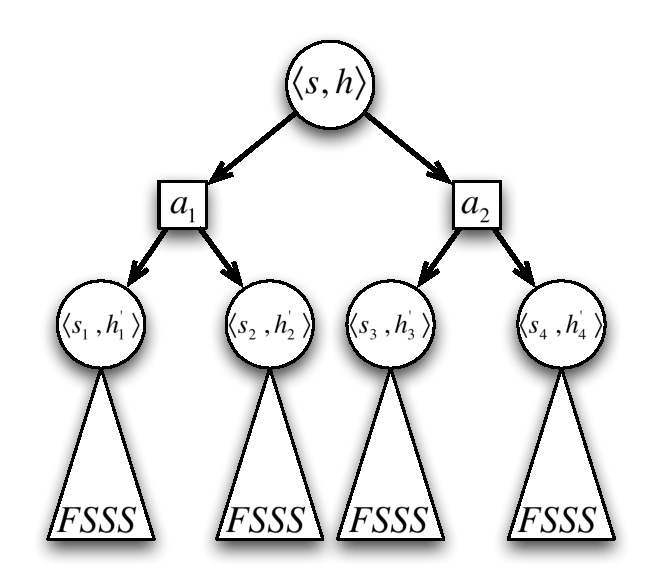
\includegraphics[scale=0.5]{figures/bfs3}}
\caption{
%{\bf Left:} the search tree when the agent is at state $s_0$ with no further observations. {\bf Right:} the agent has taken a single step in the world by performing action $a_1$, resulting in a transition to state $s_2$. White nodes indicate hypotheticals that may or may not happen. Grayed nodes indicate things that have been observed. Blackened nodes indicate data that is no longer pertinent and can be thrown out.
\alg{BFS3} samples next-belief-states for each action $C$ times, and then runs \alg{FSSS} on the resulting belief state, using the BAMDP as a generative model. Every node that is the same distance from the root represents one of the possible worlds that the agent may experience, each with a different history and MDP posterior.
}
\label{fig:bfs3}
\end{center}
\vskip -0.2in
\end{figure} 

\subsection{BFS3 is PAC-BAMDP}
\label{sec:bfs3:pac-bamdp-informal}

If certain reasonable prerequisites are satisfied, then with high probability, \alg{BFS3} will choose actions that are approximately Bayes-optimal except for a small number of times.

\begin{defn}
Let $m_\mathcal{A}$ be the MDP given to \alg{FSSS}, as described in Section~\ref{sec:bfs3:fsss-modification}, and let $\pi_t(x) = \argmax_a Q_t(x,a)$, where $Q_t$ is the upper bound on the value, as determined by \alg{FSSS} at time-step $t$.
\end{defn}

\begin{defn}
An \emph{unknown} state-action pair is one with fewer than $B$ visits. A \emph{known} state-action pair is any state-action pair with at least $B$ visits.
\end{defn}

\begin{defn}
A \emph{pinned} belief state is one with an $\epsilon_A$-accurate value according to $V_t$. That is, $|V_t(s)-V_{\mathcal{A}}(s)|\leq\epsilon_A$. It is important to note that the agent does not necessarily know which belief states are pinned.
\end{defn}

\begin{defn}
Let $C$ be the quantity such that $C$ samples from a transition function are enough to create an $\epsilon_T^C$-accurate approximation with probability at least $1-\delta_T^C$, and such that $C$ samples from a reward function are enough to create an $\epsilon_R^C$-accurate approximation with probability at least $1-\delta_R^C$. Since \alg{BFS3}'s sample complexity does not depend on a particular value for $C$, only on the accuracies and success probabilities, it is sufficient to assert that such a value for $C$ exists, without finding it, for the proof of PAC-BAMDP.
\end{defn}

\begin{thm}
\label{bfs3:proof-of-pacbamdp}
With probability at least $1-\delta$, the expected number of sub-$\epsilon$-Bayes-optimal actions taken by \alg{BFS3} is at most $BSA(S+1)d/\delta_l$ if the following assumptions are true.
\begin{enumerate}
\item
\label{theorem:cond-acc} 
Accuracy: The prior's transition function and reward function have a sample complexity of at most $B$, for a transition accuracy of $\epsilon_T$ with probability at least $1-\delta_T$, and a reward accuracy of $\epsilon_R$ with probability at least $1-\delta_R$.
\item
\label{bfs3:cond:opt}
Optimism: If running \alg{FSSS} on belief-state $x$ results in $V_t(x)> V_A(x) + \epsilon_A$ (that is, afterwards $x$ remains an unpinned belief state), then $\pi_t$ leads from $x$ through a sequence of at most $d$ unpinned belief states, ending with an unknown state-action pair, with probability at least $\delta_l$, where $d$ is the search depth used by \alg{FSSS}.
\end{enumerate}
\end{thm}

\begin{proofsketch}

First, we will show that there is a BAMDP, constructed from the prior $\phi$, whose optimal policy is the Bayes-optimal policy for $m_0\sim \phi$. Then, we will show that \alg{BFS3}, acting in the BAMDP, will satisfy the three criteria required for PAC-MDP behavior~\cite{kakade03,lihong09pacmdp} in that BAMDP\footnote{PAC-MDP behavior in the BAMDP implies near Bayes-optimal behavior in the learning setting.}.
These criteria are: \begin{inparaenum} \item accuracy, \item bounded discoveries, and \item optimism. \end{inparaenum}

First, because of Assumption~\ref{theorem:cond-acc} in our theorem statement, we know that once we have received $B$ examples of transitions from a state-action pair $(s,a)$, our estimate of the next-state distribution for that pair will be accurate.  (This condition need not hold for degenerate priors, but it appears to hold quite broadly.)

Second, since we forget all additional transitions from state-action pairs for which we have seen $B$ examples, the number of possible state-histories that an agent can observe is bounded.  Specifically, each time a transition from some state-action $(s,a)$ is observed, either no change will be made to the state-action's histogram (it already sums to $B$), or exactly one entry in the histogram will be incremented by $1$.  Since the histogram can be changed at most $B$ times, the total number of histories possible for an agent over the course of a single experiment is $B \cdot S \cdot A$ ($B$ histories for each state-action pair).

A discovery event, or one that potentially changes the MDP posterior, is an event that results in a change to the history. There are $B \cdot S \cdot A$ discoveries possible, since other transitions will be forgotten.

Third, $\mathbf{FSSS}(x',d,C,T,M_\phi)$ is guaranteed to have an optimistic value estimate for belief-state $x'$ as $T$ (the number of trajectories), our bounded resource, grows smaller. We also know that, from Assumption~\ref{bfs3:cond:opt} of the theorem, $T$ is sufficient to find accurate estimates of $x'$ if all states in $s'$'s subtree have converged next-state posteriors. Simply put, if $x'$'s subtree has no unknown state-action pairs, then \alg{FSSS}'s estimate of that state's value will be accurate.  As a result, if \alg{FSSS}'s estimate of a state's value is inaccurate, there must be something to learn about in $x'$'s subtree. \alg{FSSS} guarantees that this inaccuracy will be optimistic.

Also possible is that the value estimate of $x'$ is accurate \emph{and} there are unknown states in its subtree. In this case, the agent can decide whether or not to visit that state fully informed of its value, and can take a Bayes-optimal action.

The PAC-MDP criteria direct the agent to areas of either high value or high uncertainty, managing the exploration/exploitation tradeoff. Because the agent will only go to areas of high uncertainty over areas of high reward a bounded number of times that grows linearly with the number of possible discovery events, we bound the number of sub-optimal steps taken over the lifetime of the agent.
\end{proofsketch}


\section{Proof of PAC-BAMDP}

This section presents the detailed argument that \alg{BFS3} is near
Bayes-optimal.

There are two distinct steps to this proof. The first step is to find the likelihood that all estimates are accurate. That likelihood is then the likelihood that \alg{BFS3} will be $\epsilon$-Bayes optimal for all but a small expected number of steps. The second step is to bound that number, assuming all estimates are accurate.

\subsection{Definitions}

This section will list several definitions important to the proof.

\begin{defn}
Let $H$ be the set of all histories, which are sequences of $(s,a,r,s')$ transitions.
\end{defn}

\begin{defn}
Let $X=S\times H$ be the set of belief states.
\end{defn}

\begin{defn}
Let the BAMDP $m_\phi$ be the MDP with state space $X$, action space $A$, and the transition and reward functions:
\begin{eqnarray}
T_{m_\phi}(x'|x,a)= T_{m_\phi}(\langle s', h'\rangle|\langle s, h)\rangle, a) &=& f(h'|h,s,a) \int_m \phi(m|h)T_m(s'|s,a) dm,\\
f(h'|h,s,a) &=& \mathbb{1}[h'=h+(s,a,r,s')],\\
R_{m_\phi}(x,a) = R_{m_\phi}(\langle s, h)\rangle, a) &=& \int_m \phi(m|h) R_m(s,a).
\end{eqnarray}
That is, $m_\phi$ is the BAMDP based on the prior $\phi$.
\end{defn}

\begin{defn}
Let $n_h(s,a)$ be the number of transitions from $(s,a)$ in $h$.
\end{defn}

\begin{defn}
Let the set of possible histories $H^B \subset H$ be the set of histories with no more than $B$ examples of transitions from any state-action pair. That is, 
\begin{eqnarray}
H^B&=&\{h|h\in H\wedge \forall_{s,a} c_h(s,a) \leq B\}.
\end{eqnarray}
\end{defn}

\begin{defn}
Let the BAMDP $m_\phi^B$ be the MDP with state space $X^B = S\times H^B$, action space $A$, and the transition and reward functions:
\begin{eqnarray}
T_{m_\phi^B}(x'|x,a)= T_{m_\phi}(\langle s', h'\rangle|\langle s, h)\rangle, a) &=& f_B(h'|h,s,a) \int_m \phi(m|h)T_m(s'|s,a) dm,\\
f_B(h'|h,s,a) &=& \left\{\begin{array}{lll}
n_h(s,a)\leq B&:& \mathbb{1}[h'=h+(s,a,r,s')]\\
n_h(s,a) = B&:& \mathbb{1}[h'=h],
\end{array}\right.\\
R_{m_\phi^B}(x,a) &=& R_{m_\phi}(x, a).
\end{eqnarray}
That is, $m_\phi^B$ is the BAMDP based on the prior $\phi$, where transitions from state-action pairs with at least $B$ examples in the history are forgotten. Since the transition function has a sample complexity of $B$, with an accuracy of $\epsilon_T$, and the reward function has a sample complexity of $B$ with an accuracy of $\epsilon_R$, $m_\phi^B$ is an $\epsilon_T$, $\epsilon_R$ approximation of $m_\phi$.
\end{defn}

\begin{defn}
Let the BAMDP $m_\mathcal{A}$ be the MDP with state space $X^B = S\times H^B$, action space $A$, and the transition and reward functions $T_\mathcal{A}$ and $R_\mathcal{A}$,
where
\begin{eqnarray}
\forall_{x',x,a} |T_\mathcal{A}(x'|x,a) - T_{m_\phi^B}(x'|x,a)| &\leq& \epsilon^c_T,\\
\forall_{x,a} |R_\mathcal{A}(x,a) - R_{m_\phi^B}(x,a)| &\leq& \epsilon^c_R.
\end{eqnarray}
That is, $m_\mathcal{A}$ is an $\epsilon^c_T$, $\epsilon^c_R$ approximation of $m_\phi^B$.
\end{defn}

\subsection{Accuracy}

This section will find the likelihood that all estimates are accurate.

There are two sets of estimates to be made. The first set is the accuracy of a transition function estimate and reward function, given that estimate, given $C$ samples from the functions being estimated. We will call such an estimate a $C$-estimate.

\begin{lemma}
All $C$-estimates of the transition and reward function of $m_\phi^B$ will be $\epsilon_T^c$-accurate and $\epsilon_R^c$-accurate with probability at least $1-\delta_C$, where
\begin{eqnarray}
\delta_C &=& BS^2A^2(\delta_T^C+\delta_R^C).
\end{eqnarray}
\end{lemma}

\begin{proof}
The probability that, for a given history, state, and action, the transition and reward estimates both fall within their bounds, is at least $1-(\delta_T^C+\delta_R^C)$, by the union bound.

Since the maximum size of a history is $B S A$ (since there may be at most $B$ examples of each state-action pair), and since the history used by \alg{BFS3} will never shrink, the agent can experience at most $BSA$ histories over the course of its lifetime. For each of those histories, there are at most $SA$ state-action pairs for which it may make estimates. Multiplying those two together limits the number of history-state-action combinations at $B S^2 A^2$.

The probability that all $C$-estimates for all state-action-history combinations are correct, over the lifetime of the agent, is $1-BS^2A^2(\delta_T^C+\delta_R^C)$ by the union bound.
\end{proof}

The second set is the estimate of the posterior after $B$ examples are observed from the MDP drawn from the prior. We will call such an estimate a $B$-estimate.

\begin{lemma}
All $B$-estimates of the transition and reward function of $m_\phi$ will be $\epsilon_T$-accurate and $\epsilon_R$-accurate with probability at least $1-\delta_B$, where
\begin{eqnarray}
\delta_B &=& SA(\delta_T+\delta_R).
\end{eqnarray}
\end{lemma}

\begin{proof}
The probability that, for a given state-action pair with $B$ examples, the posterior transition and reward functions both fall within their bounds is at least $1-(\delta_T+\delta_R)$, by the union bound.

The maximum number of state-action pairs that can ever have $B$ examples is $SA$ (all of them).

The probability that all $B$-estimates for all state-action pairs are correct, over the lifetime of the agent, is $1-SA(\delta_T+\delta_R)$ by the union bound.
\end{proof}

The likelihood that all estimates of any sort are accurate needs to be established.

\begin{lemma}
\label{sec:bfs3:all-estimates}
All $C$-estimates and $B$-estimates made by \alg{BFS3} fall within their bounds with probability at least $1-\delta$, where
\begin{eqnarray}
\delta &=& BS^2A^2(\delta_T^C+\delta_R^C)+ SA(\delta_T+\delta_R).
\end{eqnarray}
\end{lemma}

\begin{proof}
Proof follows immediately from the union bound.
\end{proof}

\begin{lemma}
With probability at least $1-\delta$, $m_\mathcal{A}$ is an $\epsilon_T^C$,$\epsilon_R^C$-approximation of $m_\phi^B$, and $m_\phi^B$ is an $\epsilon_T$,$\epsilon_R$-approximation of $m_\phi$.
\end{lemma}

\begin{proof}
Since the estimates whose probabilities are bounded by Lemma~\ref{sec:bfs3:all-estimates} are exactly those estimates used to create $m_\phi^B$ and $m_\mathcal{A}$, when those estimates hold, the bounds between those MDPs hold as well.
\end{proof}

\subsection{Bounded sub-optimality}

This section presents bounds between the value of a state in $m_\mathcal{A}$ and $m_\phi$, and then shows that \alg{BFS3} will take only a small number of sub-optimal steps in $m_\mathcal{A}$ and, therefore, a small number of sub-optimal steps in $m_\phi$.


\begin{lemma}
The difference in the values of the two MDPs $m_{\mathcal{A}}$ and $m_\phi$ for a given state is bounded by the Simulation Lemma.
\begin{eqnarray}
|V_{m_\mathcal{A}}(s) - V_{m_\phi}(s)| &\leq& s(\epsilon_T+\epsilon^c_T,\epsilon_R+\epsilon^c_R),\\
|Q_{m_\mathcal{A}}(s,a) - Q_{m_\phi}(s,a)| &\leq& s(\epsilon_T+\epsilon^c_T,\epsilon_R+\epsilon^c_R),\\
s(\epsilon_T+\epsilon^c_T,\epsilon_R+\epsilon^c_R) &=& \frac {(\epsilon_R+\epsilon^c_R) + \gamma \Vmax(\epsilon_T+\epsilon^c_T)} {1-\gamma}.
\end{eqnarray}
\end{lemma}
\begin{proof}
Since $m_\mathcal{A}$ is an $\epsilon^c_T$, $\epsilon^c_R$ approximation of $m_\phi^B$, and $m_\phi^B$ is an $\epsilon_T$, $\epsilon_R$ approximation of $m_\phi$, $m_\mathcal{A}$ is an $(\epsilon_T+\epsilon^c_T)$, $(\epsilon_R+\epsilon^c_R)$ approximation of $m_\phi$. Proof follows immediately from the Simulation Lemma.
\end{proof}

\begin{lemma}
Acting near-optimally in $m_\mathcal{A}$ is sufficient for acting near-optimally in $m_\phi$. 
Specifically, an action that is $\epsilon_A$-optimal in $m_\mathcal{A}$ is $\epsilon$-optimal in $m_\phi$, where $\epsilon_A=\epsilon - s(\epsilon_T+\epsilon^c_T,\epsilon_R+\epsilon^c_R)$.
\end{lemma}
\begin{proof}
Proof is immediate.
\end{proof}

Since an action that is $\epsilon_A$-optimal in $m_\mathcal{A}$ is $\epsilon$-optimal in $m_\phi$, we will bound the number of sub-$\epsilon_A$-optimal steps in $m_\mathcal{A}$.



\begin{defn}
A \emph{model discovery} is the event where the agent visits an unknown state-action pair.
\end{defn}

\begin{defn}
A \emph{value discovery} is the event where \alg{BFS3} plans and causes a belief state to become pinned.
\end{defn}

\begin{defn}
A \emph{policy epoch} is a sequence $n$ steps long starting at $t$, where $\forall_{0<i\leq n} \pi_t = \pi_i$. That is, a policy epoch is a time period during which the policy does not change.
\end{defn}

\begin{defn}
A \emph{history epoch} is a sequence of steps without a model discovery.
\end{defn}

\begin{defn}
The agent's estimate of the value of belief-state $x$ at time step $t$ is $V_t(x)$. Since \alg{BFS3} will use the estimates from the previous time-step as a way to boot-strap its current estimates, we define $V_{-1}(x)=\Vmax$.
\end{defn}

Every time \alg{BFS3} visits a belief state for the first time in a given policy epoch, it will run \alg{FSSS} at most $CA$ times, using each of the at most $CA$ possible next belief states as the roots. \alg{FSSS} will reuse and overwrite the previous value estimates, such that if \alg{BFS3} runs \alg{FSSS} on belief-state $x$ at step $t$, \alg{FSSS} will start with the upper bound on the value of each belief state at $V_{t-1}(x)$, and an equivalent memory for the lower bound. After \alg{FSSS} is done, $V_t(x)$ is the new upper-bound estimate for $x$.

The following is the proof of Theorem~\ref{bfs3:proof-of-pacbamdp}
\begin{proof}
Let $m_\mathcal{A}^h$ be the set of belief states in $m_\mathcal{A}$ with the history $h$. Once an agent leaves $m_\mathcal{A}^h$ it can never return, since the only way $h$ can change is by growing bigger.

The strategy will be to show that when \alg{BFS3} enters $m_\mathcal{A}^h$, the number of sub-$\epsilon_A$-optimal actions it takes before leaving is small. The time starting when \alg{BFS3} enters this set of states and leaves is a history epoch.

The number of possible model discoveries during a history epoch is $1$, since making a discovery ends the epoch.

The number of possible value discoveries during a history epoch is $S$, since there are at most $S$ possible belief states in the set $m_\mathcal{A}^h$, and by the consistency condition, a value discovery can be made once per belief state. In addition, after $S$ value discoveries in a history epoch, all remaining steps in that history epoch will be $\epsilon_A$-optimal, since all states have $\epsilon_A$-accurate values.

Since, at step $t$, \alg{BFS3} will either replan or the policy will remain unchanged since the last time the agent visited belief-state $x_t$, either $\argmax_a Q_A(x_t,a)$ is $\epsilon_A$-optimal, or the current policy $\pi_t$ will reach an unknown state-action pair in the next $d$ steps with probability at least $\delta_l$.

If $\argmax_a Q_A(x_t,a)$ is not $\epsilon_A$-optimal, with probability at least $\delta_l$, the agent will either make a model discovery (if all the $d$ belief states in the sequence remain unknown) or a value discovery (if \alg{BFS3} replans during the sequence and figures out the $\epsilon_A$-accurate value).

The total number of possible model discovery and value discovery events during a history epoch, when combined, numbers no more than $S+1$ (there are $S$ possible value discoveries, and one possible model discovery). Since every $d$-step window beginning at a belief state with inaccurate $Q$-values has a probability of at least $\delta_l$ of making one of these $S+1$ discoveries, the expected number of sub-$\epsilon_A$-optimal steps per history epoch is at most $(S+1)d/\delta_l$.

Since there are at most $BSA$ history epochs, one per possible model discovery, the expected number of sub-$\epsilon_A$-optimal steps for the lifetime of the agent is at most $BSA(S+1)d/\delta_l$.
\end{proof}

%
\ifperchapterbib%
For the convenience of the reader, a list of references is provided at the end of each chapter (where applicable).
\ifendbib%
%A bibliography containing all cited references is included at the \hyperref[sec:bibliography]{end of the dissertation}.
\else\fi% end ifendbib
%\cbend%
\else\fi% end ifperchapterbib
